\chapter{为什么要开课?}

\paragraph*{先来个练习}让我们从下面这篇虚构的文章开始(不必关注它所涉的背景知识)。这篇文章包含了一些排印错误,或者说一些用法的错误 
    \footnote{不像拼写有正字法,法文没有官方的“排印规则”,取而代之的是建议、步骤等(参见第 \ref{chap8} 章的参考资料)。然而,尽管不同作者的用法不尽相同,这些用法之间也十分相似。可以说,一些用法已经达成了共识!}
。你能找到几处错误?

\begin{figure}
    \centering
    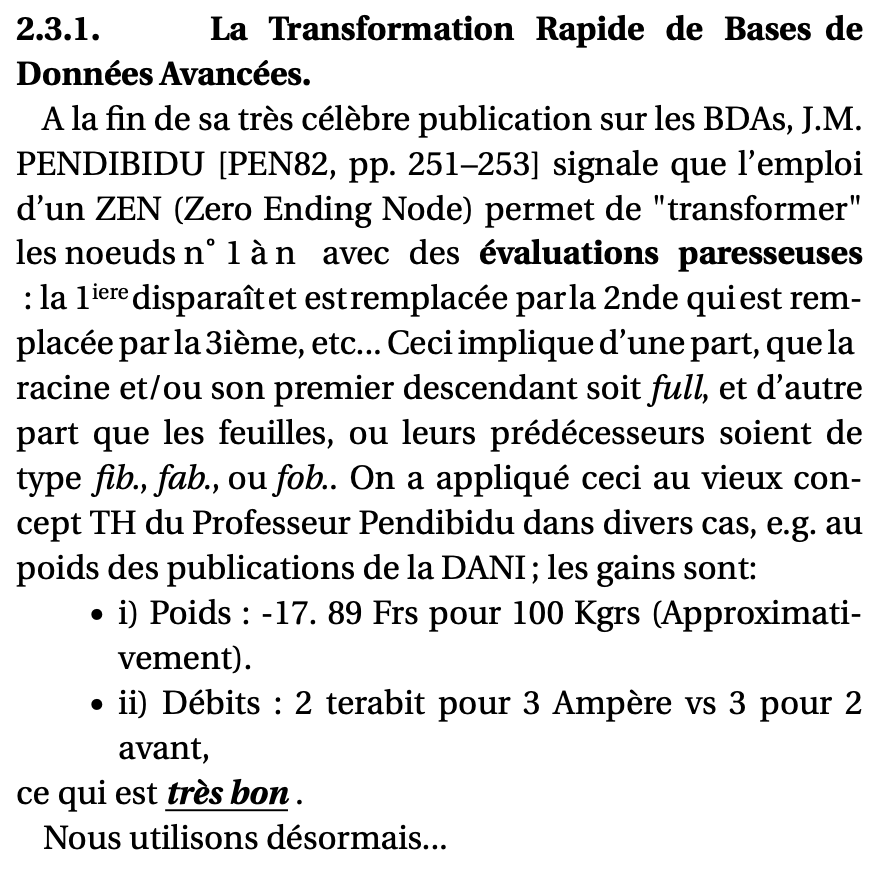
\includegraphics[width = \linewidth]{img/1.png}

\begin{mdframed}
    \footnotesize
    \textbf{2.3.1 \quad 高级数据库的快速转换.}\\
    J.M. PENDIBIDU [PEN82, pp. 251-253]在其关于BDAs的著作的结尾指出,使用ZEN(Zero Ending Node)可以通过\textbf{懒评估}来\verb|"|转换\verb|"|节点n° 1到n:
    1$^{\rm iere}$消失了,被2nde取代,而2nde又被3ième取代,等等……
    这一方面意味着根和/或它的第一个后代为\emph{full},另一方面意味着叶节点或其前代的类型是\emph{fib.}、\emph{fab.}或\emph{fob.}.
    我们在不同的情况下将其应用于Pendibidu教授的旧概念TH,例如DANI的出版物重量;结果如下:\\
    $\cdot$ i) 重量:-17. 89 Frs每100 Kgrs(约).\\
    $\cdot$ ii) 流量:对于3安培为2太位vs之前为3、2,\\
    这种结果\textbf{\emph{\underline{非常好}}}.\\
    现在,我们用……
\end{mdframed}

    \caption{组织得很糟糕的文字}
    \label{fig1}
\end{figure}

如果你将这样的文章直接发给仍然带有编辑部门的学术期刊,如《信息科学技术》(\emph{Technique et Science Informatiques,TSI}),你将收到如图\ref{fig2}所示的校样,并且期刊会要求重新整理稿件。

\begin{figure}
    \centering
    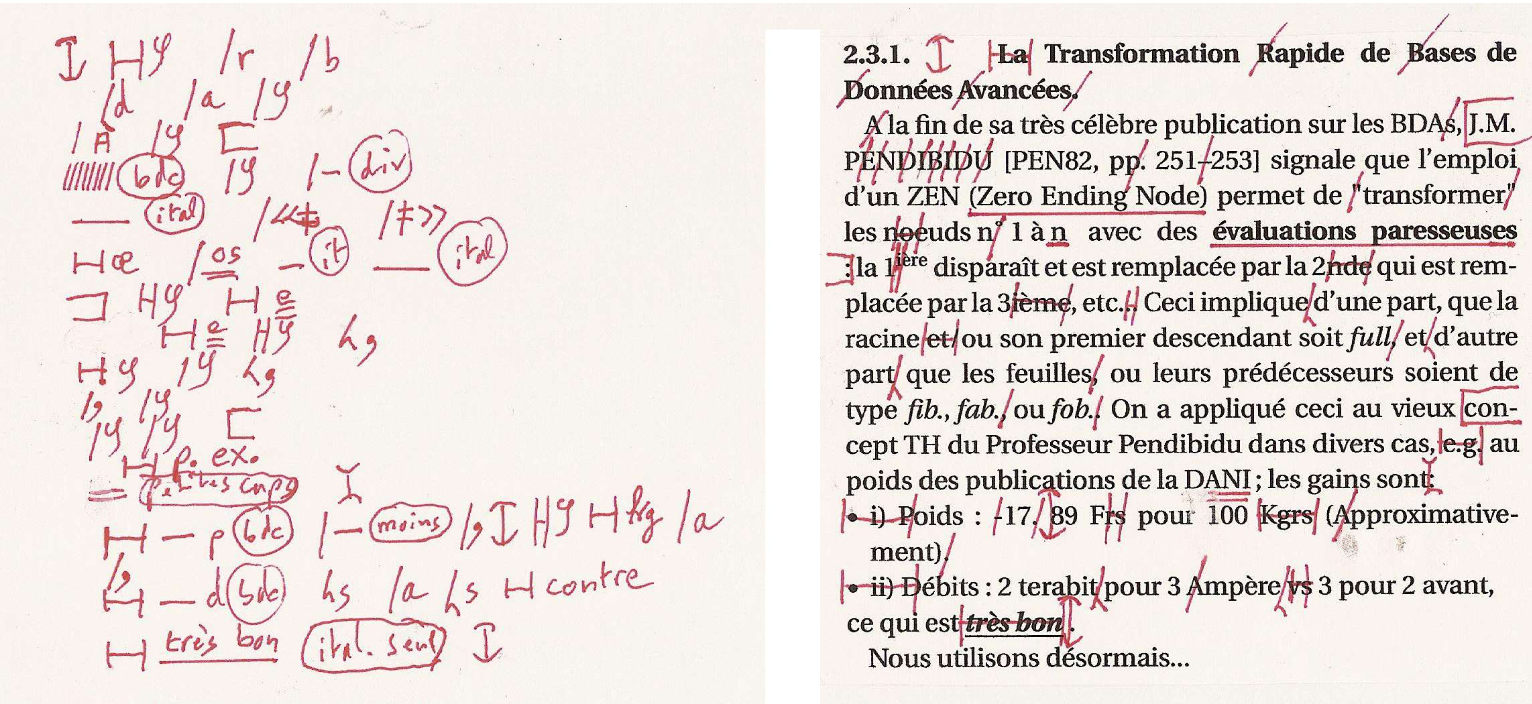
\includegraphics[width = \linewidth]{img/2.png}
    \caption{图\ref{fig1}中的文字,带有校对符号}
    \label{fig2}
\end{figure}

在这里,我们不会为你提供上面练习的详细解答,因为它会非常长。但我们会在下面列出一些具有代表性的差错(校对标记就代表了差错,其更正形式见图\ref{fig3}),并在图\ref{fig3}中以更好的方式呈现了这一小段文字。图\ref{fig1}中的文字有以下经典错误:

\begin{itemize}
    \item 标题:
    \begin{itemize}
        \item 标题一般不加冠词;
        \item 标题不采用各单词首字母大写的形式;
        \item 标题结尾不加句点。
    \end{itemize} 
    \item 第1行:
    \begin{itemize}
        \item 大写字母应当添加变音符号(见\ref{sec3.2}节);
        \item 首字母缩写不应带复数(见\ref{sec2.3}节);
        \item 不在姓名中间换行(见\ref{sec5.1.3}小节)。
    \end{itemize}
    \item 第2行:
    \begin{itemize}
        \item 专有名词不应全大写;
        \item 表示页码的缩写应当是“p.”(见\ref{sec2.3}节)。
    \end{itemize}
    \item 第3行:
    \begin{itemize}
        \item 外语单词连带其两侧的圆括号应当设为意大利体(见\ref{sec4.6}节);
        \item 法文的引号应当为双楔形的«...»形式(见\ref{sec2.2}节)。
    \end{itemize}
    \item 第4行:
    \begin{itemize}
        \item noeud的正确拼写形式应当为nœud;
        \item numéro的缩写应当使用上角字母o(n$^{\rm o}$)而此处使用了度的符号(n°),且需要添加代表复数的$^{\rm s}$。
    \end{itemize}
    \item 第5行:
    \begin{itemize}
        \item 冒号应当位于上一行;
        \item 第1和第3的缩写应当分别为$1^{\rm re}$和$3^{\rm e}$(见\ref{sec2.3}节),但最好是写出全称,且此处的seconde应当使用deuxième。
    \end{itemize}
    \item ……
\end{itemize}

\begin{figure}
    \centering
    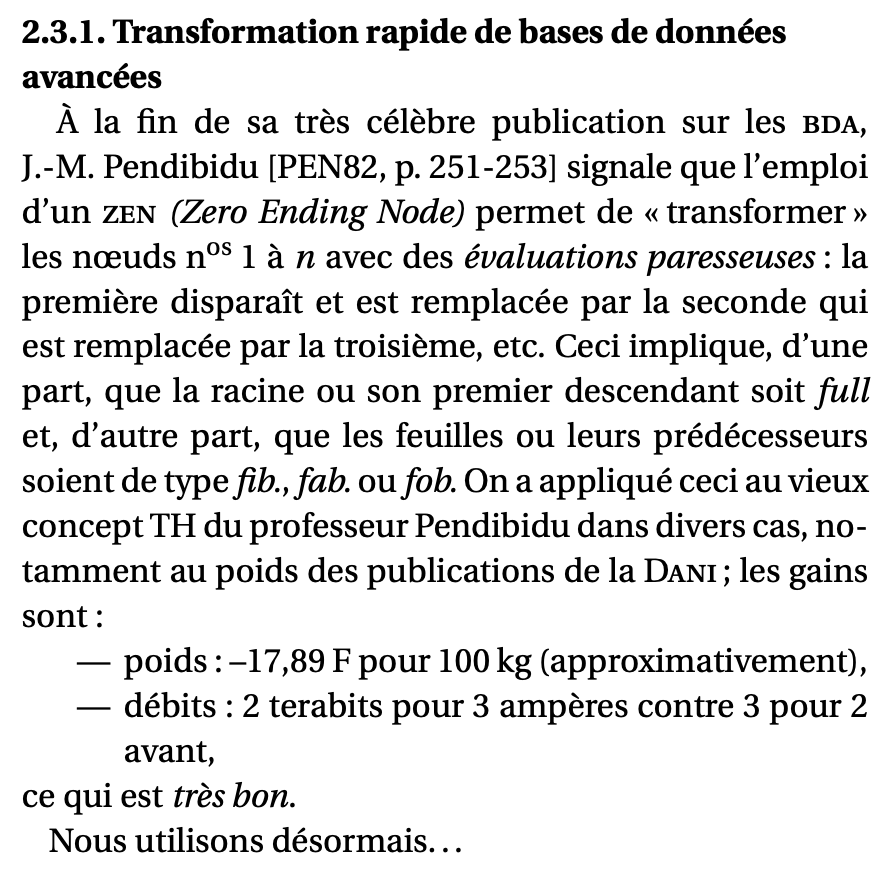
\includegraphics[width = \linewidth]{img/3.png}

\begin{mdframed}
    \footnotesize
    \textbf{2.3.1 \quad 高级数据库的快速转换}\\
    J.M. Pendibidu [PEN82, p. 251-253]在其关于\textsc{bda}的著作的结尾指出,使用\textsc{zen}\emph{(Zero Ending Node)}可以通过\emph{懒评估}来«转换»节点n$^{\rm os}$ 1到$n$:
    第1个节点消失了,被第2个取代,而第2个又被第3个取代,等等。
    这一方面意味着,根或它的第一个后代为\emph{full},另一方面意味着,叶节点或其前代的类型是\emph{fib.}、\emph{fab.}或\emph{fob.}。
    我们在不同的情况下将其应用于Pendibidu教授的旧概念TH,例如\textsc{Dani}的出版物重量;结果如下:\\
    \mbox{\qquad} ---  重量:$-17,89$ F每100 kg(约数),\\
    \mbox{\qquad} ---  流量:对于3安培为2太位,对比之前为3、2,\\
    这种结果\emph{非常好}。\\
    现在,我们用……
\end{mdframed}

    \caption{与图\ref{fig1}相同的文字,合入图\ref{fig2}的校对符号}
    \label{fig3}
\end{figure}

按理说
    \footnote{我使用了这个短语的现代写法:À priori。见\ref{sec4.6}}
,我们想指出,这并不是在钻牛角尖(尤其是已经攒了这么多出来)。然而,看看修改过的版本(图\ref{fig3})就可以发现,文本更可读了、表达更精准了。遵循这些排印规则不需要什么成本,去了解和应用它们也是如此。

然而,为什么会出现这么多错误呢?事实表明,研究人员越来越多地自己撰写文章或报告,可是他们很少接受的文书方面的培训,也就会经常忽略拼写和排印错误。此外,科技出版在过去(实际上也没有过去多少年),不论是从内容是形式上讲,都出自专业之手——内容上,有期刊编辑委员会、大会科学委员会等来把关;形式上,有文字编辑部门来把关——不像今天,任何人都可以通过\emph{网络}来随便写些什么东西。在那样的形势下,完好呈现出来的文件,无论是印刷品还是显示在屏幕上,实际上都在发行之前被掘地三尺地编校过。例如,在IRISA(Institut de Recherche en Informatique et Systèmes Aléatoires,计算机科学和随机系统研究所)1989年的活动报告中,平均每页被找出6个差错。至于硕士生写出来的大小论文……好吧,这些作者都已经有一些排印(typographie)的基础知识了
    \footnote{或者说\emph{正字法(orthotypographie)}知识,除了字体、版式等内容外,还包含了使用正确的正字符号,而这也是排印的一部分。}
。

这个小课堂的目的是促使我的同事
    \footnote{鉴于他们都是计算机科学家或自动化专家,我的例子往往更贴这些领域。}
更好地把控他们的出版物中的文字,以提升其质量。

以下所有内容都与任何排版引擎无关
    \footnote{尽管我认为\LaTeX (也就是这个文档所使用的排版引擎)对于科技文本来说更适合,无论针对纸质内容还是\emph{网络}内容,但我还是要指出,有个东西叫MS Word。}
,也不涉及任何美观的问题(如何选择字体、如何选择布局等,见参考文献)%TODO
。最后,这些内容同时适用于印刷和屏幕显示。